\chapter{Πρακτική Υλοποίηση \& Παραδείγματα Μαθημάτων}
\label{chap:implementation}

Στο παρόν κεφάλαιο η τεχνική ανάλυση του Κεφαλαίου~\ref{chap:standards} μεταφέρεται στο επίπεδο πραγματικών πακέτων περιεχομένου. Αντί για αφηρημένη περιγραφή των προδιαγραφών, εξετάζονται επιλεγμένα παραδείγματα από τη συλλογή \ENG{Golf Examples}~\cite{SCORMGolfExamples}, ώστε να φανεί πώς το \ENG{manifest}, ο μηχανισμός \ENG{run-time} και οι κανόνες \ENG{sequencing} υλοποιούνται σε κώδικα και σε κανονικά αρχεία μαθήματος.

Η ενότητα δεν επιχειρεί πλήρη καταγραφή όλων των διαθέσιμων δειγμάτων. Επιλέγονται μόνο όσα λειτουργούν ως αντιπροσωπευτικές περιπτώσεις για το \ENG{SCORM} 1.2 και το \ENG{SCORM} 2004, ώστε το κεφάλαιο να παραμείνει σύντομο και ταυτόχρονα να διατηρεί σαφή σύνδεση με τα τεχνικά συμπεράσματα του προηγούμενου κεφαλαίου.

\section{Επισκόπηση Παραδειγμάτων Μαθημάτων}
\label{sec:example_courses_overview}

Η συλλογή \ENG{Golf Examples} χρησιμοποιείται ευρέως ως υλοποίηση αναφοράς για τη δοκιμή και την κατανόηση πακέτων \ENG{SCORM}, επειδή κάθε παράδειγμα απομονώνει ένα συγκεκριμένο τεχνικό χαρακτηριστικό του προτύπου~\cite{SCORMGolfExamples}. Για τους σκοπούς της παρούσας εργασίας επιλέγονται τέσσερα πακέτα: τα \ENG{\path{ContentPackagingSingleSCO_SCORM12.zip}} και \ENG{\path{RuntimeMinimumCalls_SCORM12.zip}} για το \ENG{SCORM} 1.2, καθώς και τα \ENG{\path{RuntimeMinimumCalls_SCORM20043rdEdition.zip}} και \ENG{\path{SequencingForcedSequential_SCORM20043rdEdition.zip}} για το \ENG{SCORM} 2004.

Η επιλογή αυτή δεν είναι τυχαία. Το πρώτο ζεύγος αντιστοιχεί άμεσα στις δύο βασικές διαστάσεις του \ENG{SCORM} 1.2 που αναλύθηκαν στις Ενότητες~\ref{subsec:scorm12_cam} και~\ref{subsec:scorm12_rte}, δηλαδή στο πακετάρισμα περιεχομένου και στην \ENG{run-time} επικοινωνία. Το δεύτερο ζεύγος επιτρέπει να φανεί πώς το \ENG{SCORM} 2004 διατηρεί τον ίδιο βασικό μηχανισμό εκκίνησης, αλλά τον επεκτείνει με πλουσιότερο μοντέλο δεδομένων και με τυπικό \ENG{sequencing}, όπως περιγράφηκε στις Ενότητες~\ref{subsec:scorm2004_rte} και~\ref{subsec:scorm2004_sn}.

Πέρα από την τεχνική τους αξία, τα παραδείγματα αυτά είναι χρήσιμα και επειδή το περιεχόμενό τους παραμένει οπτικά απλό. Οι σελίδες \ENG{HTML}, οι εικόνες και τα \ENG{JavaScript} αρχεία δεν κρύβουν την προδιαγραφή πίσω από βαρύ εκπαιδευτικό σχεδιασμό· αντίθετα, την καθιστούν ευανάγνωστη. Έτσι, ο αναγνώστης μπορεί να συνδέσει με σχετική ευκολία τις αφηρημένες έννοιες του Κεφαλαίου 3 με πραγματικά αρχεία, πραγματικά \ENG{identifiers} και πραγματικές κλήσεις μέσω \ENG{API}.

\subsection{Ενδεικτικό οπτικό υλικό από το περιεχόμενο}
\label{subsec:golf_example_visuals}

Το ίδιο το μαθησιακό περιεχόμενο των \ENG{Golf Examples} αποτελείται από απλές σελίδες \ENG{HTML} που συνοδεύονται από στατικές εικόνες και κοινά αρχεία μορφοποίησης. Τα αρχεία αυτά δηλώνονται ρητά στο \ENG{\texttt{imsmanifest.xml}} και φορτώνονται ως μέρος των αντίστοιχων \ENG{resources}. Το Σχήμα~\ref{fig:golf_example_content} παρουσιάζει τρεις χαρακτηριστικές εικόνες από το περιεχόμενο των ενοτήτων \ENG{Playing}, \ENG{Etiquette} και \ENG{Handicapping}, οι οποίες περιλαμβάνονται αυτούσιες στα πακέτα.

\begin{figure}[htbp]
\centering
\begin{subfigure}[t]{0.31\textwidth}
    \centering
    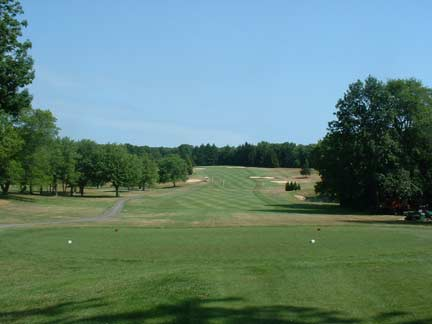
\includegraphics[width=\linewidth]{chapters/04_Example_Courses/figures/golf_playing.jpg}
    \caption{\ENG{Playing}}
\end{subfigure}
\hfill
\begin{subfigure}[t]{0.31\textwidth}
    \centering
    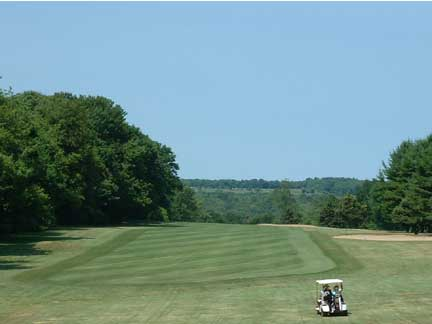
\includegraphics[width=\linewidth]{chapters/04_Example_Courses/figures/golf_course.jpg}
    \caption{\ENG{Etiquette}}
\end{subfigure}
\hfill
\begin{subfigure}[t]{0.31\textwidth}
    \centering
    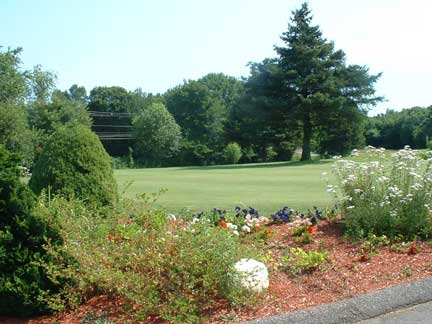
\includegraphics[width=\linewidth]{chapters/04_Example_Courses/figures/golf_handicapping.jpg}
    \caption{\ENG{Handicapping}}
\end{subfigure}
\caption{Ενδεικτικές εικόνες από το περιεχόμενο των \ENG{Golf Examples}}
\label{fig:golf_example_content}
\end{figure}

Η παρατήρηση αυτή έχει πρακτική σημασία. Οι εικόνες του Σχήματος~\ref{fig:golf_example_content} δεν αποτελούν εξωτερικό διακοσμητικό υλικό, αλλά τυπικούς πόρους περιεχομένου που δηλώνονται μέσα στο πακέτο, συνδέονται με συγκεκριμένα \ENG{HTML} αρχεία και συμμετέχουν στο ίδιο συμβόλαιο φορητότητας που αναλύθηκε στο Κεφάλαιο 3. Με άλλα λόγια, ακόμη και το απλό οπτικό υλικό υπάγεται στην ίδια λογική αυτοτέλειας του \ENG{PIF} και του \ENG{manifest}.

\section{Παράδειγμα Μαθήματος \ENG{SCORM} 1.2}
\label{sec:scorm12_example}

Η πρακτική αποτύπωση του \ENG{SCORM} 1.2 βασίζεται σε δύο συμπληρωματικά πακέτα της συλλογής \ENG{Golf Examples}: το \ENG{\path{ContentPackagingSingleSCO_SCORM12.zip}}, το οποίο δείχνει την ελάχιστη μορφή πακεταρίσματος, και το \ENG{\path{RuntimeMinimumCalls_SCORM12.zip}}, το οποίο προσθέτει τον απολύτως βασικό κύκλο ζωής επικοινωνίας με το \ENG{LMS}. Ο συνδυασμός τους είναι ιδιαίτερα χρήσιμος, επειδή επιτρέπει να φανεί στην πράξη ότι το \ENG{SCORM} 1.2 συγκροτείται από δύο διακριτές αλλά αλληλένδετες διαστάσεις: το \ENG{CAM} και το \ENG{RTE}.

\subsection{Πακετάρισμα και \ENG{\texttt{imsmanifest.xml}}}
\label{subsec:scorm12_manifest}

Στο επίπεδο του πακεταρίσματος, το \ENG{SCORM} 1.2 παράδειγμα επιβεβαιώνει σχεδόν κατά λέξη τα συμπεράσματα της Ενότητας~\ref{subsec:scorm12_cam}. Η οργάνωση του μαθήματος εκφράζεται μέσω των στοιχείων \ENG{\texttt{<organization>}} και \ENG{\texttt{<item>}}, ενώ οι πραγματικοί πόροι δηλώνονται χωριστά στην ενότητα \ENG{\texttt{<resources>}}. Το ακόλουθο απόσπασμα από το \ENG{\path{RuntimeMinimumCalls_SCORM12.zip}} είναι χαρακτηριστικό, επειδή συνδέει έναν λογικό κόμβο πλοήγησης με έναν εκτελέσιμο πόρο και τα συνοδευτικά του αρχεία.

{\selectlanguage{english}\fontencoding{T1}\selectfont
\begin{lstlisting}[language=XML, caption={Απόσπασμα \ENG{manifest} από το \ENG{RuntimeMinimumCalls\_SCORM12}}, label={lst:ch4_scorm12_manifest}]
<item identifier="playing_par_item" identifierref="playing_par_resource">
  <title>Par</title>
</item>

<resource identifier="playing_par_resource"
          type="webcontent"
          adlcp:scormtype="sco"
          href="Playing/Par.html">
  <file href="Playing/Par.html"/>
  <file href="Playing/par.jpg"/>
  <dependency identifierref="common_files" />
</resource>
\end{lstlisting}
}

Το απόσπασμα αυτό αναδεικνύει τρία σημεία που συνδέονται άμεσα με την προηγούμενη τεχνική ανάλυση. Πρώτον, το \ENG{\texttt{identifierref}} λειτουργεί ως ο σύνδεσμος ανάμεσα στη λογική δομή και στον πραγματικό πόρο, όπως ακριβώς περιγράφηκε κατά την ανάλυση της σχέσης \ENG{organizations/resources}. Δεύτερον, η τιμή \ENG{\texttt{adlcp:scormtype="sco"}} δηλώνει ότι το αρχείο \ENG{\texttt{Playing/Par.html}} δεν είναι απλό \ENG{asset}, αλλά μονάδα εκτέλεσης με πρόσβαση στο \ENG{API}. Τρίτον, η ύπαρξη \ENG{\texttt{dependency}} προς το \ENG{\texttt{common\_files}} δείχνει πώς η προδιαγραφή επιτρέπει την κοινή χρήση \ENG{JavaScript}, \ENG{CSS} και βοηθητικών αρχείων χωρίς διπλασιασμό πόρων.

Στην ίδια λογική, οι εικόνες που παρουσιάστηκαν στο Σχήμα~\ref{fig:golf_example_content} δηλώνονται ρητά ως \ENG{\texttt{<file>}} στοιχεία μέσα στα αντίστοιχα \ENG{resources}. Αυτό είναι τεχνικά σημαντικό, επειδή αποδεικνύει ότι ακόμη και τα πιο απλά αρχεία περιεχομένου εντάσσονται στην ίδια συμβατική περιγραφή φορητότητας που καθορίζει το \ENG{manifest}.

\subsection{Ελάχιστος κύκλος ζωής \ENG{Run-Time}}
\label{subsec:scorm12_api}

Η ουσιώδης μετάβαση από απλό πακέτο περιεχομένου σε πραγματικό \ENG{SCO} γίνεται στο \ENG{\path{RuntimeMinimumCalls_SCORM12.zip}}, όπου προστίθεται το κοινό αρχείο \ENG{\path{shared/scormfunctions.js}}. Το παράδειγμα είναι σκόπιμα λιτό: δεν επιδιώκει να δείξει όλες τις δυνατότητες του μοντέλου δεδομένων, αλλά μόνο τον ελάχιστο μηχανισμό εντοπισμού του \ENG{API} και τον ορθό κύκλο ζωής αρχικοποίησης και τερματισμού.

{\selectlanguage{english}\fontencoding{T1}\selectfont
\begin{lstlisting}[language=JavaScript, caption={Ελάχιστος \ENG{SCORM} 1.2 \ENG{run-time} κύκλος ζωής}, label={lst:ch4_scorm12_runtime}]
function ScormProcessInitialize(){
    API = getAPI();
    if (API == null){ return; }

    var result = API.LMSInitialize("");
    if (result == SCORM_FALSE){ return; }

    initialized = true;
}

function ScormProcessFinish(){
    if (initialized == false || finishCalled == true){ return; }

    var result = API.LMSFinish("");
    finishCalled = true;
}

window.onload = ScormProcessInitialize;
window.onunload = ScormProcessFinish;
window.onbeforeunload = ScormProcessFinish;
\end{lstlisting}
}

Το συγκεκριμένο μοτίβο επιβεβαιώνει ακριβώς όσα αναλύθηκαν στην Ενότητα~\ref{subsec:scorm12_rte}. Το \ENG{SCO} πρέπει πρώτα να εντοπίσει το αντικείμενο \ENG{\texttt{API}} στην ιεραρχία παραθύρων, στη συνέχεια να καλέσει τη \ENG{\texttt{LMSInitialize("")}} πριν από οποιαδήποτε άλλη ενέργεια και, τέλος, να τερματίσει τη συνεδρία με \ENG{\texttt{LMSFinish("")}}. Η χρήση και των \ENG{onunload} και \ENG{onbeforeunload} είναι επίσης ενδεικτική των ιστορικών περιορισμών του προτύπου, το οποίο βασίζεται σε εύθραυστο \ENG{browser-side} κύκλο ζωής και γι' αυτό απαιτεί αμυντικό προγραμματισμό ακόμη και για την ελάχιστη συμμόρφωση.

Ιδιαίτερο ενδιαφέρον έχει το ότι το παράδειγμα δεν καλεί καθόλου \ENG{\texttt{LMSSetValue()}}. Αυτό δεν αποτελεί έλλειψη, αλλά σκόπιμη σχεδιαστική επιλογή: αποδεικνύει ότι η ελάχιστη συμβατή εκτέλεση στο \ENG{SCORM} 1.2 είναι η δημιουργία, διατήρηση και ορθή λήξη της συνεδρίας. Με άλλα λόγια, πριν ακόμη εξεταστούν στοιχεία όπως \ENG{\texttt{cmi.core.lesson\_status}} ή \ENG{\texttt{cmi.suspend\_data}}, η ίδια η ύπαρξη έγκυρου \ENG{session lifecycle} είναι το βασικό συμβόλαιο συνεργασίας μεταξύ περιεχομένου και \ENG{LMS}.

\subsection{Σύντομη αποτίμηση}
\label{subsec:scorm12_summary}

Το \ENG{SCORM} 1.2 παράδειγμα δείχνει με καθαρό τρόπο ότι η τεχνική απλότητα του προτύπου δεν σημαίνει απουσία αυστηρότητας. Το πακέτο παραμένει φορητό επειδή το \ENG{\texttt{imsmanifest.xml}} περιγράφει με σαφήνεια τη δομή και τους πόρους του, ενώ η εκτέλεση παραμένει διαλειτουργική επειδή κάθε \ENG{SCO} τηρεί τον ελάχιστο κύκλο ζωής του \ENG{API}. Η πρακτική εικόνα που προκύπτει συμφωνεί πλήρως με το Κεφάλαιο 3: η ισχύς του \ENG{SCORM} 1.2 προέρχεται κυρίως από την απλή αλλά σταθερή τυποποίηση πακεταρίσματος και εκκίνησης.

\section{Παράδειγμα Μαθήματος \ENG{SCORM} 2004}
\label{sec:scorm2004_example}

Για το \ENG{SCORM} 2004 επιλέγονται δύο παραδείγματα με διαφορετικό ρόλο. Το \ENG{\path{RuntimeMinimumCalls_SCORM20043rdEdition.zip}} αποτυπώνει την ελάχιστη προσαρμογή του \ENG{run-time} μοντέλου από το \ENG{SCORM} 1.2 προς το αντικείμενο \ENG{\texttt{API\_1484\_11}} και τις μεθόδους \ENG{\texttt{Initialize()}} / \ENG{\texttt{Terminate()}}. Το \ENG{\path{SequencingForcedSequential_SCORM20043rdEdition.zip}}, αντίθετα, δείχνει πώς η βασική αυτή λογική επεκτείνεται με \ENG{bookmarking}, διακριτή παρακολούθηση ολοκλήρωσης και επιτυχίας, καθολικά \ENG{objectives} και δηλωτικούς κανόνες \ENG{sequencing}.

\subsection{\ENG{Run-Time} συμπεριφορά και εμπλουτισμένο μοντέλο δεδομένων}
\label{subsec:scorm2004_runtime_example}

Η πιο χαρακτηριστική διαφορά του \ENG{SCORM} 2004 στο επίπεδο της πραγματικής εκτέλεσης δεν είναι μόνο η μετονομασία του \ENG{API}, αλλά η πιο ρητή χρήση του μοντέλου δεδομένων. Στο \ENG{\path{shared/launchpage.html}} του παραδείγματος \ENG{\path{SequencingForcedSequential_SCORM20043rdEdition.zip}}, η λογική εκκίνησης και πλοήγησης γράφεται απευθείας πάνω σε στοιχεία όπως \ENG{\texttt{cmi.completion\_status}}, \ENG{\texttt{cmi.location}} και \ENG{\texttt{cmi.success\_status}}.

{\selectlanguage{english}\fontencoding{T1}\selectfont
\begin{lstlisting}[language=JavaScript, caption={Παράδειγμα \ENG{SCORM} 2004 \ENG{runtime} παρακολούθησης}, label={lst:ch4_scorm2004_runtime}]
var completionStatus = ScormProcessGetValue("cmi.completion_status", true);
if (completionStatus == "unknown"){
    ScormProcessSetValue("cmi.completion_status", "incomplete");
}

var bookmark = ScormProcessGetValue("cmi.location", false);

ScormProcessSetValue("cmi.location", currentPage);

if (currentPage == (pageArray.length - 1)){
    reachedEnd = true;
    ScormProcessSetValue("cmi.completion_status", "completed");

    if (hasAssessment == false){
        ScormProcessSetValue("cmi.success_status", "passed");
    }

    ScormProcessCommit();
}
\end{lstlisting}
}

Το απόσπασμα αυτό συνδέεται άμεσα με την ανάλυση της Ενότητας~\ref{subsec:scorm2004_rte}. Ο διαχωρισμός ανάμεσα σε \ENG{\texttt{cmi.completion\_status}} και \ENG{\texttt{cmi.success\_status}} γίνεται πραγματικός μηχανισμός ελέγχου της μαθησιακής κατάστασης. Παράλληλα, το \ENG{\texttt{cmi.location}} αξιοποιείται ως σημείο συνέχισης, ενώ η ρητή κλήση \ENG{\texttt{Commit()}} υποδηλώνει ότι η κατάσταση του \ENG{runtime} πρέπει να καθίσταται διαθέσιμη εγκαίρως και προς το υποσύστημα \ENG{sequencing}.

Το ίδιο παράδειγμα δείχνει και την πιο στενή σύνδεση ανάμεσα στο \ENG{runtime} και στην πλοήγηση. Κατά την έξοδο, ο κώδικας γράφει \ENG{\texttt{cmi.exit="suspend"}} και θέτει \ENG{\texttt{adl.nav.request="suspendAll"}} ή \ENG{\texttt{adl.nav.request="exitAll"}}, ανάλογα με το αν ο χρήστης θέλει να συνεχίσει αργότερα ή να ολοκληρώσει οριστικά την εκτέλεση. Έτσι, η πλοήγηση παύει να είναι μόνο ζήτημα διεπαφής \ENG{LMS} και μετατρέπεται σε τυπικό μέρος της συμβατικής επικοινωνίας που ορίζει το \ENG{SCORM} 2004.

\subsection{\ENG{Sequencing} και καθολικά \ENG{objectives} στο \ENG{\texttt{manifest}}}
\label{subsec:scorm2004_sequencing}

Η ουσιαστική υπεροχή του \ENG{SCORM} 2004 γίνεται ορατή στο \ENG{\texttt{imsmanifest.xml}} του \ENG{\path{SequencingForcedSequential_SCORM20043rdEdition.zip}}. Εκεί η λογική προώθησης του εκπαιδευόμενου δηλώνεται ρητά μέσω \ENG{sequencing rules} και χαρτογράφησης στόχων.

{\selectlanguage{english}\fontencoding{T1}\selectfont
\begin{lstlisting}[language=XML, caption={Κανόνας \ENG{forced sequential} στο \ENG{SCORM} 2004 \ENG{manifest}}, label={lst:ch4_scorm2004_sequencing}]
<item identifier="etiquette_item" identifierref="etiquette_resource">
  <title>Etiquette</title>
  <imsss:sequencing IDRef="common_seq_rules">
    <imsss:sequencingRules>
      <imsss:preConditionRule>
        <imsss:ruleConditions conditionCombination="any">
          <imsss:ruleCondition
            referencedObjective="previous_sco_satisfied"
            operator="not" condition="satisfied"/>
          <imsss:ruleCondition
            referencedObjective="previous_sco_satisfied"
            operator="not" condition="objectiveStatusKnown"/>
        </imsss:ruleConditions>
        <imsss:ruleAction action="disabled"/>
      </imsss:preConditionRule>
    </imsss:sequencingRules>
    <imsss:objectives>
      <imsss:objective objectiveID="previous_sco_satisfied">
        <imsss:mapInfo
          targetObjectiveID="...playing_satisfied"
          readSatisfiedStatus="true"
          writeSatisfiedStatus="false"/>
      </imsss:objective>
    </imsss:objectives>
  </imsss:sequencing>
</item>
\end{lstlisting}
}

Το παραπάνω τμήμα είναι ουσιαστικά η πρακτική μορφή των εννοιών που αναλύθηκαν στην Ενότητα~\ref{subsec:scorm2004_sn}. Ο κόμβος \ENG{Etiquette} παραμένει ορατός στο δέντρο του μαθήματος, αλλά καθίσταται \ENG{disabled} όσο δεν έχει ικανοποιηθεί ή ακόμη και αναγνωριστεί ο στόχος του προηγούμενου \ENG{SCO}. Η πληροφορία αυτή προκύπτει από ρητή δήλωση \ENG{preConditionRule} πάνω σε \ENG{objective} που διαβάζεται μέσω \ENG{mapInfo} από άλλο τμήμα του \ENG{activity tree}.

Το παράδειγμα αναδεικνύει επίσης την αξία των καθολικών \ENG{objectives}. Η ικανοποίηση του προηγούμενου \ENG{SCO} αποθηκεύεται σε κοινό στόχο, τον οποίο μπορεί να διαβάσει ο επόμενος κόμβος για να αποφασίσει αν θα ενεργοποιηθεί. Με αυτόν τον τρόπο, η κατάσταση παύει να είναι τοπική ιδιότητα ενός μόνο \ENG{SCO} και μετατρέπεται σε δεδομένο που τροφοδοτεί τη συνολική ροή του μαθήματος.

\subsection{Σύντομη αποτίμηση}
\label{subsec:scorm2004_example_summary}

Τα παραδείγματα του \ENG{SCORM} 2004 επιβεβαιώνουν ότι το πρότυπο αξιοποιεί λεπτομερέστερα στοιχεία κατάστασης, η πλοήγηση συνδέεται τυπικά με το \ENG{adl.nav} \ENG{namespace} και το \ENG{\texttt{manifest}} αποκτά ενεργό ρόλο στη ρύθμιση της μαθησιακής ακολουθίας. Έτσι, η αυξημένη εκφραστικότητα που περιγράφηκε θεωρητικά στο Κεφάλαιο 3 εμφανίζεται εδώ ως πραγματική, εκτελέσιμη λογική πάνω σε συγκεκριμένα αρχεία και συγκεκριμένες κλήσεις \ENG{API}.

